\chapter{Methodology}
\label{chap:chap2}
This project has been divided into three main sections based on the factors of unreliability mentioned earlier in \hyperref[chap:chap1]{Chapter 1}. 
The main factors studied in this project are:
\begin{itemize}
    \item Label Bias and Environmental Datashift
    \item Suitable Algorithm Selection
    \item Reward Hacking
\end{itemize}

\section{Label Bias and Environmental Datashift}
To investigate the effect of biased data labelling, we will train two models using a single independent algorithm. 
One will use biased data while the other uses unbiased data. 
These datasets will be modelled using the mathematical framework outlined in the conference paper \textit{‘Identifying and Correcting Label Bias in Machine Learning’} \cite{Jiang}. 
Each model will be trained and evaluated using data that has been split from the same distribution. 
For a model to be considered reliable, it must be able to properly generalise or adapt well to new and unseen data. 
A good, reliable model can achieve high accuracy (among other metrics) scores with low variance between datasets. 
Therefore, both of these trained models will then be fed previously unseen data (i.e. deployment data) to determine its ability to generalise.

\section{Suitable Algorithm Selection}
As shown in Figure (2.1), when it comes to AI and ML, the appropriacy of solutions or algorithms depends on elements such as the specific application and the level of supervision required. 
More often than not, more than one algorithm could be a viable solution (see \hyperref[fig:algor]{Figure 2.2}). 
Therefore, to investigate suitable algorithm selections, models will be trained with a single dataset using different algorithms (with different assumptions). 
They will then be tested for accuracy to determine suitable algorithm choices. Evaluating the reliability of a model is dependant on the model type. 
Accuracy, precision and recall are three common metrics we can use to evaluate a model. 
However, depending on particular applications, other complex means of metric evaluation may be necessary. 

\begin{figure}[h]
    \centering
    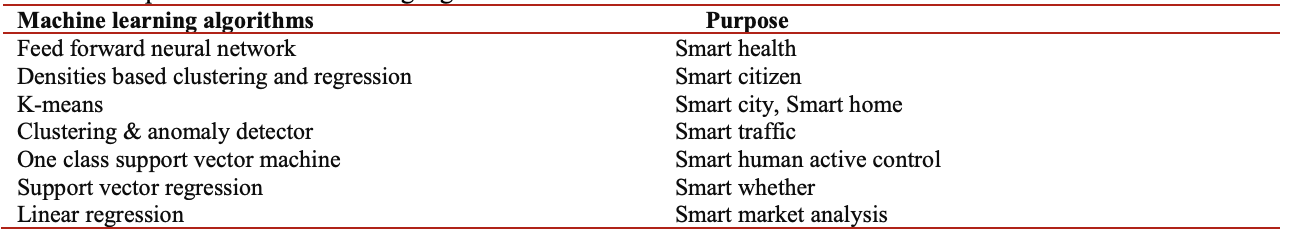
\includegraphics[width=1\textwidth]{ML_algorithms.png}
    \caption{Machine Learning Algorithms for specific applications \cite{Mohapatra}}
    \label{fig:applic}
\end{figure}

The bias-variance trade-off should be considered when optimising ML models. 
Bias is the $\text{model}'\text{s}$ ability to learn the wrong things due to oversimplification or incorrect assumptions. 
Variance is the error due to sensitivity as a result of small fluctuations in training data. 
As the complexity of the model increases, bias decreases but, the variance will increase. 
This is the trade-off between these two factors. 
An overfit model is one that is too complex, resulting in high variance and low bias, while an underfit model has low variance and high bias due to its simplistic nature. 
Both overfit and underfit models are undesirable and it is ideal to find a suitable trade-off between bias and variance (hence complexity) to yield a well fit model capable of adapting to different datasets \cite{Jedamski}. 

\begin{figure}[H]
    \centering
    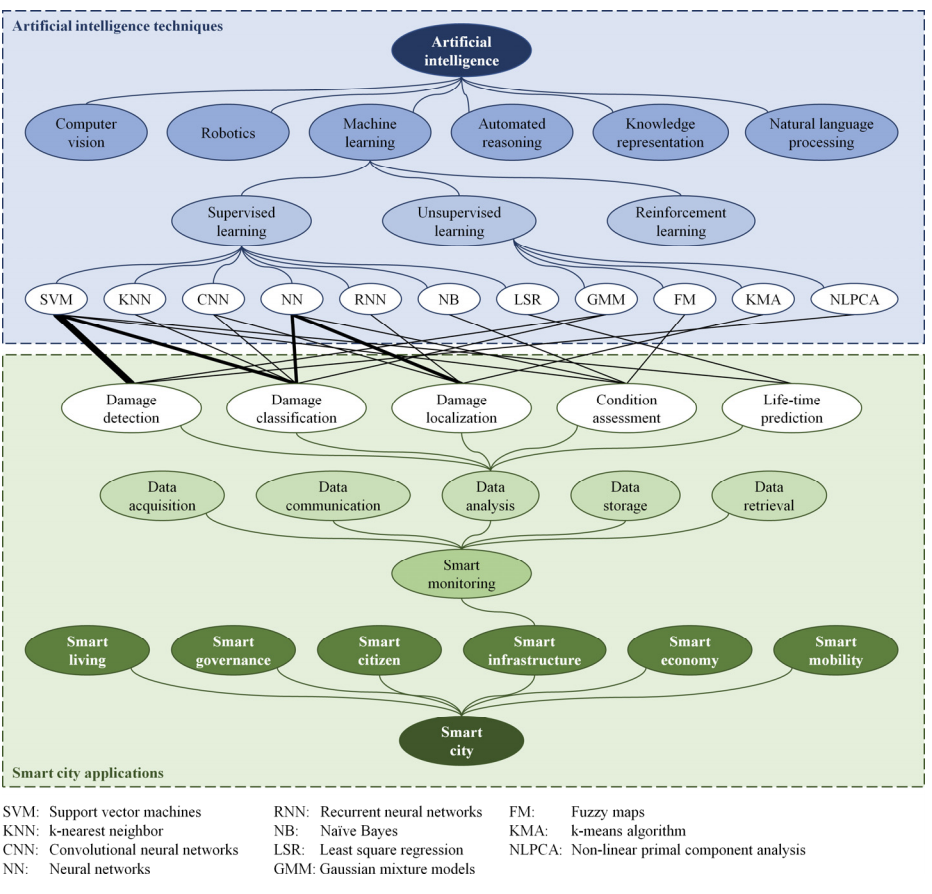
\includegraphics[width=\textwidth]{smart_monitoring_algorithms.png}
    \caption{Available ML algorithms for smart monitoring \cite{inproceedings}}
    \label{fig:algor}
\end{figure}

\enlargethispage{\baselineskip}
The dataset/s to be used in the above experiments will be obtained through various open-source data collections available online. 
Therefore, data collection is not a part of this project.
To ensure validity during the training of models, the data distribution will be split into three smaller datasets for training, validation and testing. 
The training set is used to train the models to fit the data and are evaluated against the validations set. 
The validation set being unseen, allows us to determine which models are generalising well to new examples. 
After the best model has been selected it is again tested on the test dataset as a final check on its generalisation ability. 
The training set accounts for 60\% of the complete data set, while the validation and test sets account for 20\% respecitvely. 

\section{Reward Hacking}
The two unreliability factors discussed in the above experiments are concerned mainly with supervised learning models. 
A major reliability issue within reinforcement learning models is reward hacking. 
We will perform a systematic literature review on applications and known causes of unreliability due to reward hacking as well as potential solutions.
